\chapter{Robot minisumo}

W niniejszym rozdziale opisany został proces tworzenia robota minisumo. Wyróżniono w nim trzy główne sekcje: \textit{Konstrukcja}, \textit{Elektronika} oraz \textit{Oprogramowanie}.

\begin{figure}[H]
	\centering
		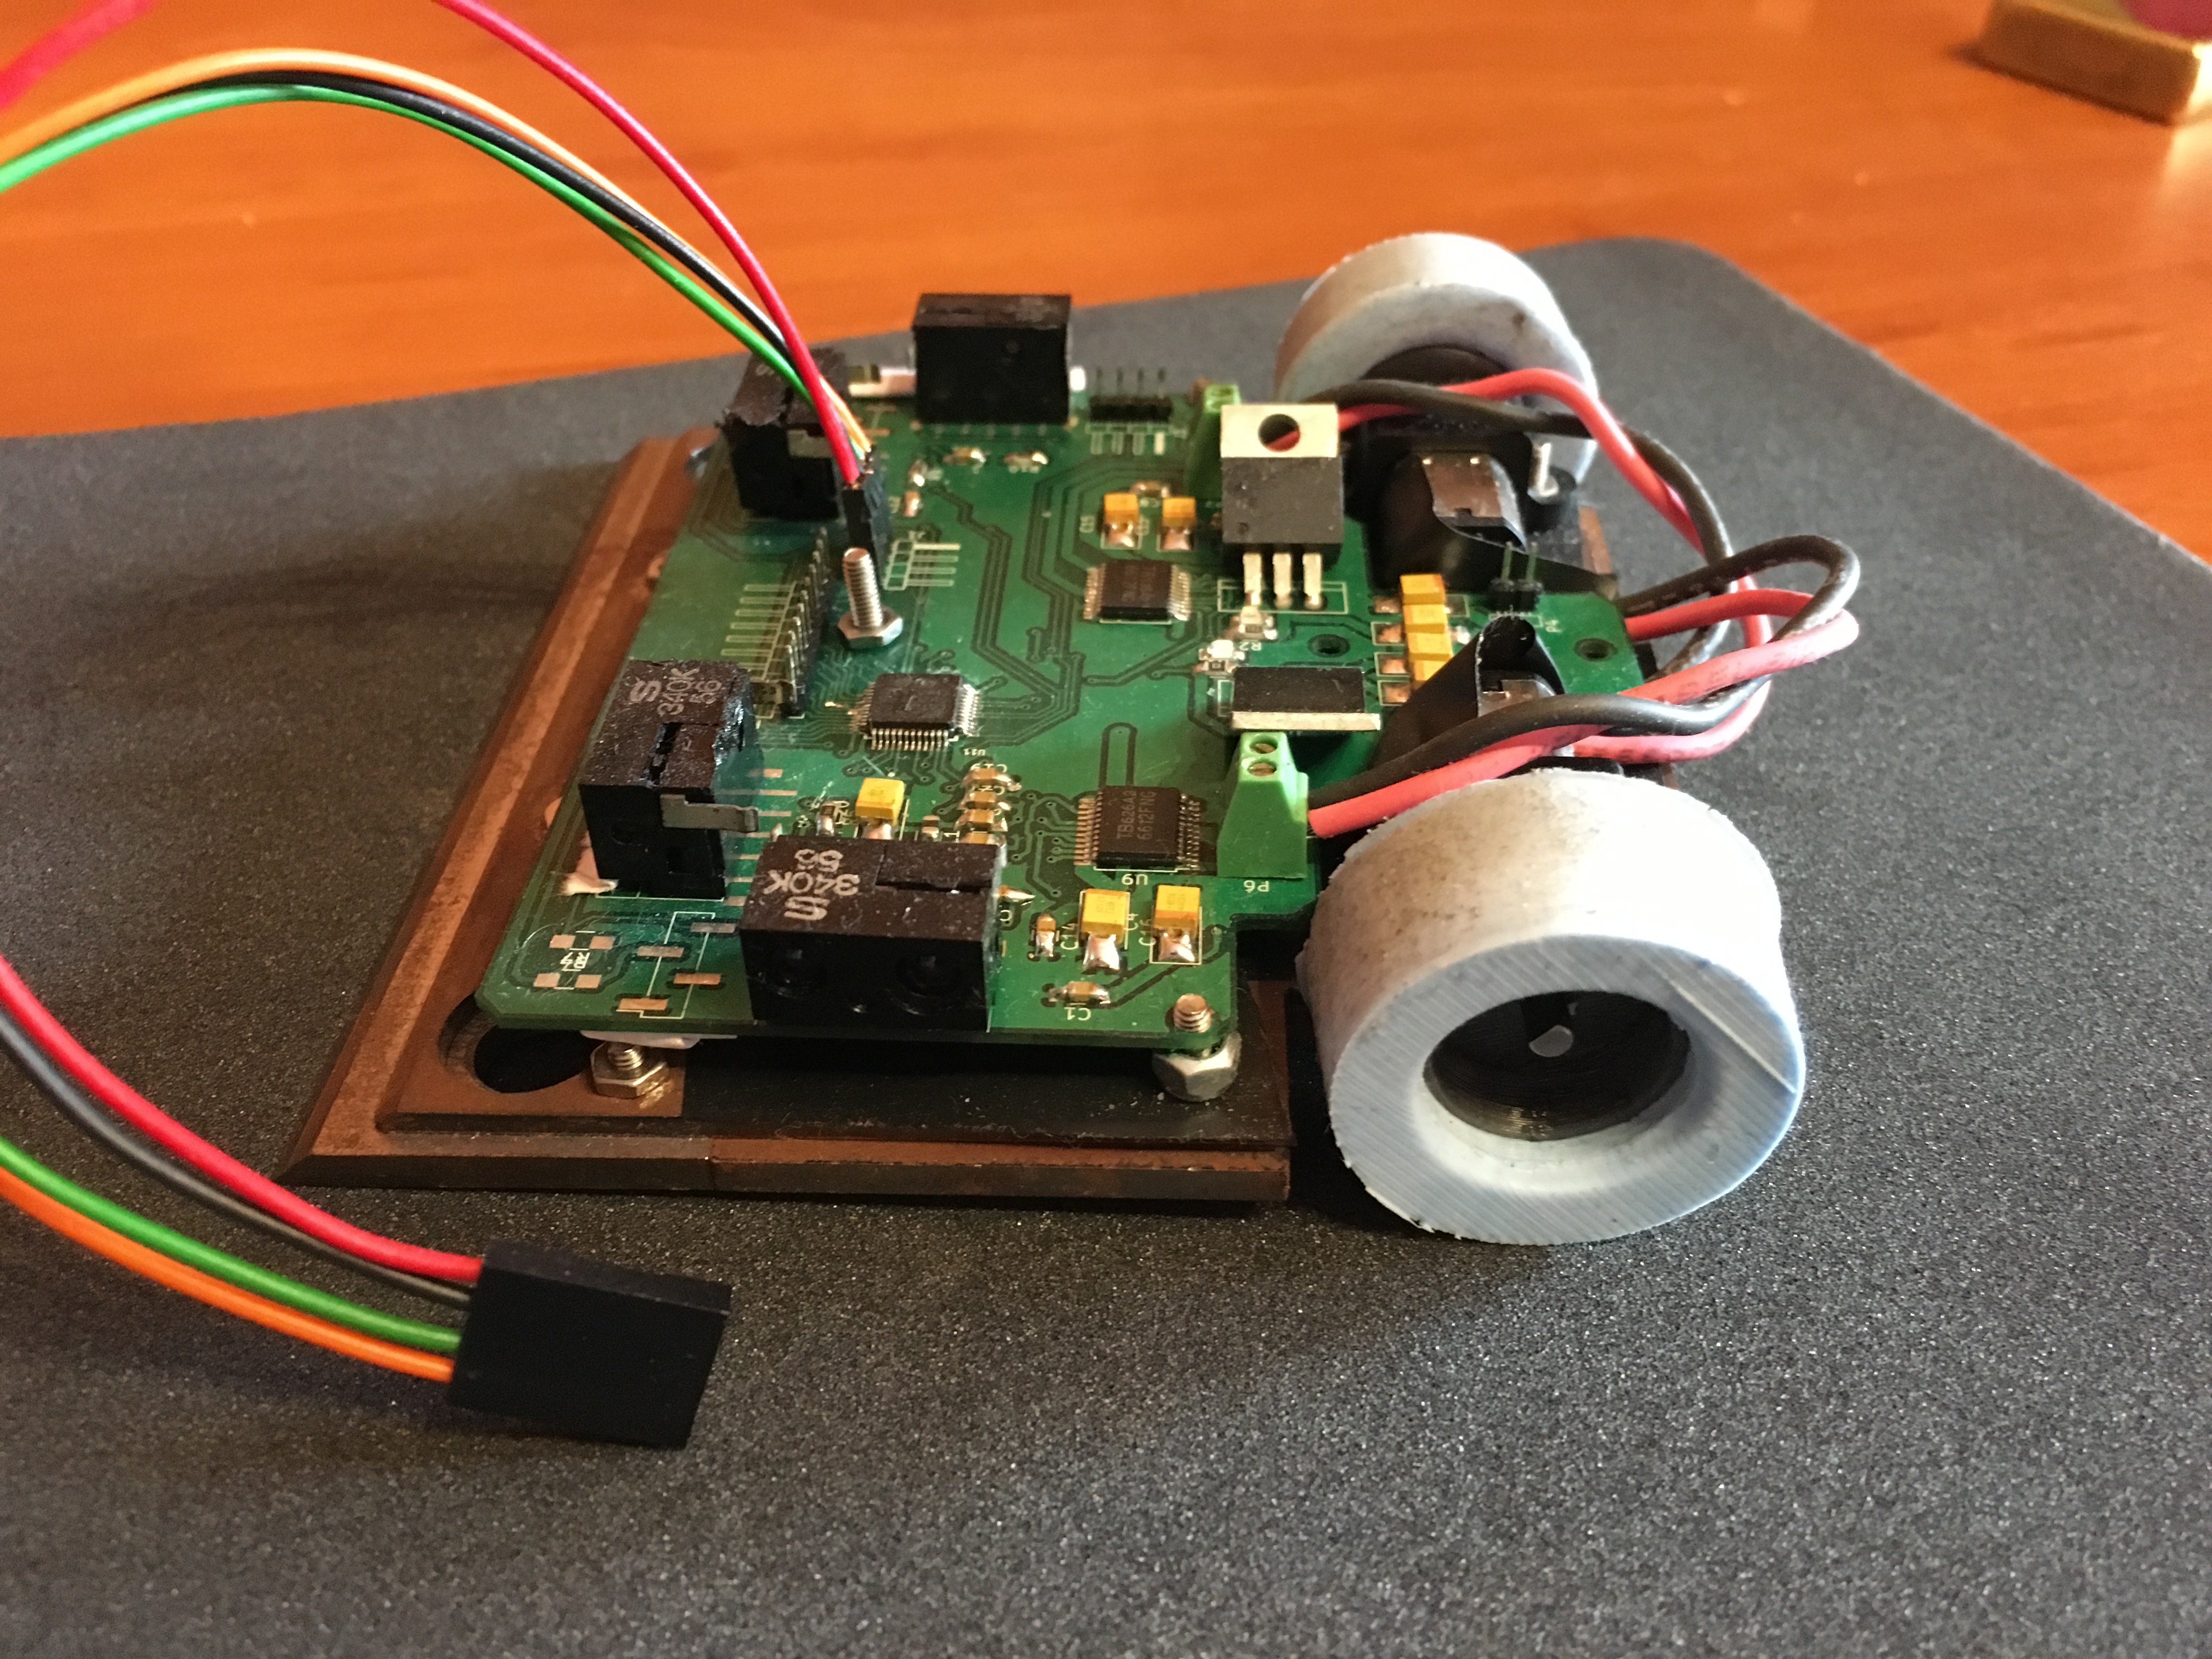
\includegraphics[width=0.75\linewidth]{pic04/minisumo.JPG}
	\caption{Wykonany robot minisumo.}
	\label{fig:robot}	
\end{figure}

Zdjęcie ~\ref{fig:robot} przedstawia omawianego robota minisumo. W celu ukazania elektroniki ściągnięto nadwozie.

\section{Konstrukcja}
\subsection{Założenia}
Głównym założeniem konstrukcyjnym było zminimalizowanie szansy podbicia robota przez przeciwnika. W związku z czym napęd robota składa się z dwóch kół umiejscowionych w tylnej części konstrukcji. Przednia część robota zakończona jest pługiem, który bezpośrednio dotyka podłoża. Dodatkowo starano się, aby środek ciężkości całej konstrukcji znajdował się jak najbliżej podłoża.

\subsection{Nadwozie}
Konstrukcja nadwozia została zaprojektowana przy użyciu środowiska \textit{Autodesk Inventor 2017}. Wybór został podyktowany łatwością obsługi narzędzi oraz darmową licencją studencką. Obudowa została wykonana w technologii druku 3D, ze względu na małą masę, koszt produkcji, oraz możliwość łatwego dostosowania do potrzeb projektu (otwory na śruby oraz czujniki przeciwnika, przestrzeń na koła).  

\begin{figure}[H]
	\centering
		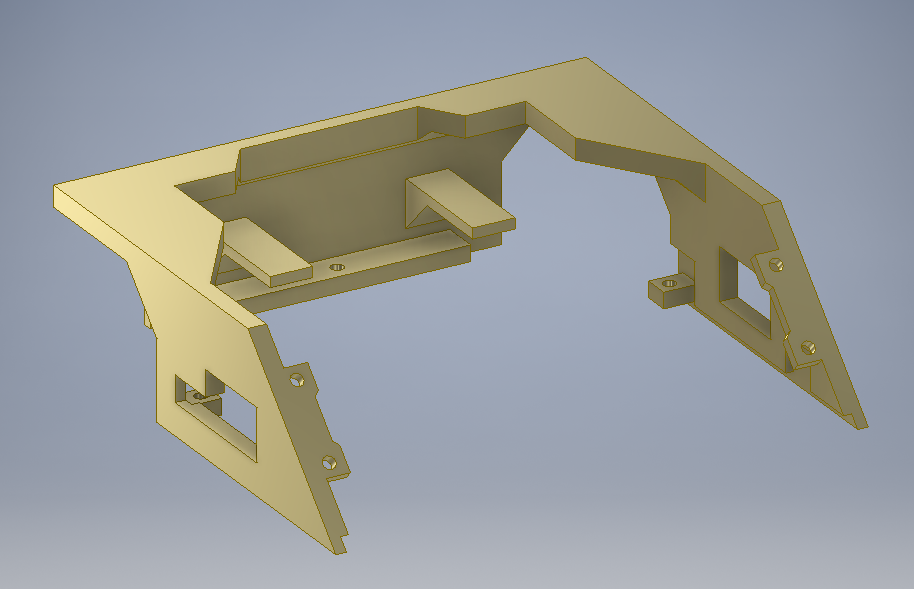
\includegraphics[width=0.75\linewidth]{pic04/body.png}
	\caption{Projekt nadwozia w środowisku Autodesk Inventor 2017.}
	\label{fig:body}	
\end{figure}

Na ilustracji ~\ref{fig:body} znajduje się projekt nadwozia robota. Ze względu na niewielką wytrzymałość plastikowego wydruku przywiązano dużą wagę do szerokości obudowy. Starano się, aby była możliwie jak najszersza, co skutkowało wzrostem trwałości całej konstrukcji. Dodatkowo front robota został wykonany ze stali, ponieważ w przypadku podważenia przeciwnika jest obszarem najbardziej podatnym na zniszczenia. 

\subsection{Podwozie}
Całość podwozia wykonana została ze stali ze względu na wytrzymałość oraz dużą masę, która przyczyniła się do znacznego obniżenia środka ciężkości całej konstrukcji.  Podobnie jak w przypadku nadwozia projekt został stworzony w środowisku \textit{Autodesk Inventor 2017}. Konstrukcja składa się z trzech płytek, z czego jedna zawiera ostrze od strugarki, wykonane z węglika spiekanego. Materiał ten cechuje się wysoką wytrzymałością oraz większą odpornością na kruszenie w porównaniu do zwykłej stali. 

\begin{figure}[H]
	\centering
		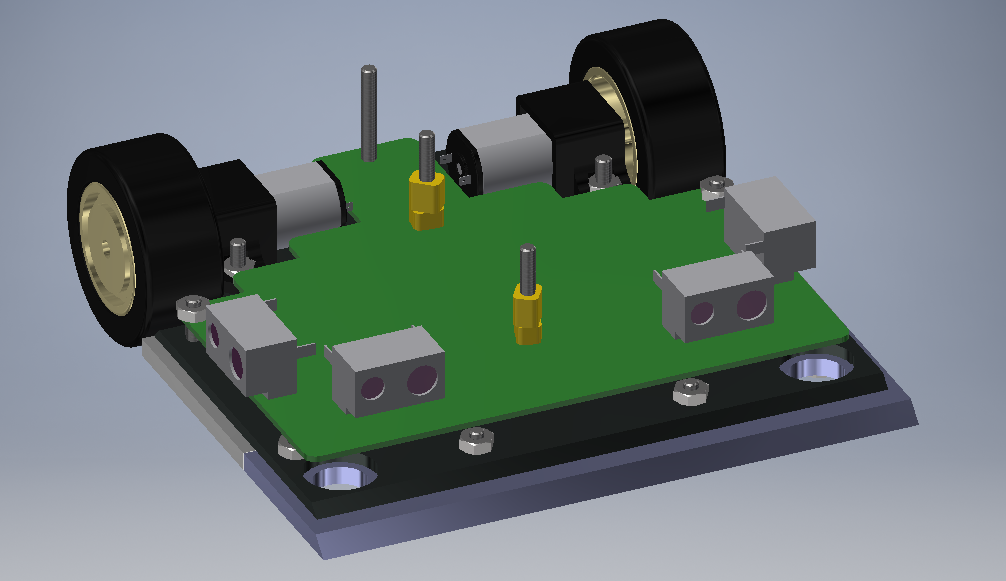
\includegraphics[width=0.75\linewidth]{pic04/chassis.png}
	\caption{Projekt podwozia w środowisku Autodesk Inventor 2017.}
	\label{fig:chassis}	
\end{figure}

Ilustracja ~\ref{fig:chassis} ukazuje wizualizację podwozia wraz z silnikami oraz kołami. Projekt wyeksportowano do formatu 2D, a następnie odpowiednie kształty wraz z otworami zostały wykonane przy użyciu techniki wypalania laserem. 

\subsection{Napęd}
Jak wspomniano wcześniej, napęd robota składa się z dwóch kół, które sterowane są niezależnie. Ruch robota wzorowany jest na zasadzie działania czołgu. W przypadku skrętu, do jednego z silników dostarczany jest większy prąd, co skutkuje wzrostem prędkości kątowej napędzanego koła. Z powodu różnicy prędkości robot zaczyna skręcać. Zdecydowano się na takie rozwiązanie ze względu na dozwoloną masę (większa ilość kół oraz silników znacząco zwiększyłaby masę całej konstrukcji) oraz manewrowość – dzięki zastosowaniu omawianego rozwiązania możliwy jest obrót robota w miejscu (w przypadku, gdy koła kręcą się w przeciwne strony), dzięki czemu pojazd jest szybki oraz zwinny. 

\begin{figure}[H]
	\centering
		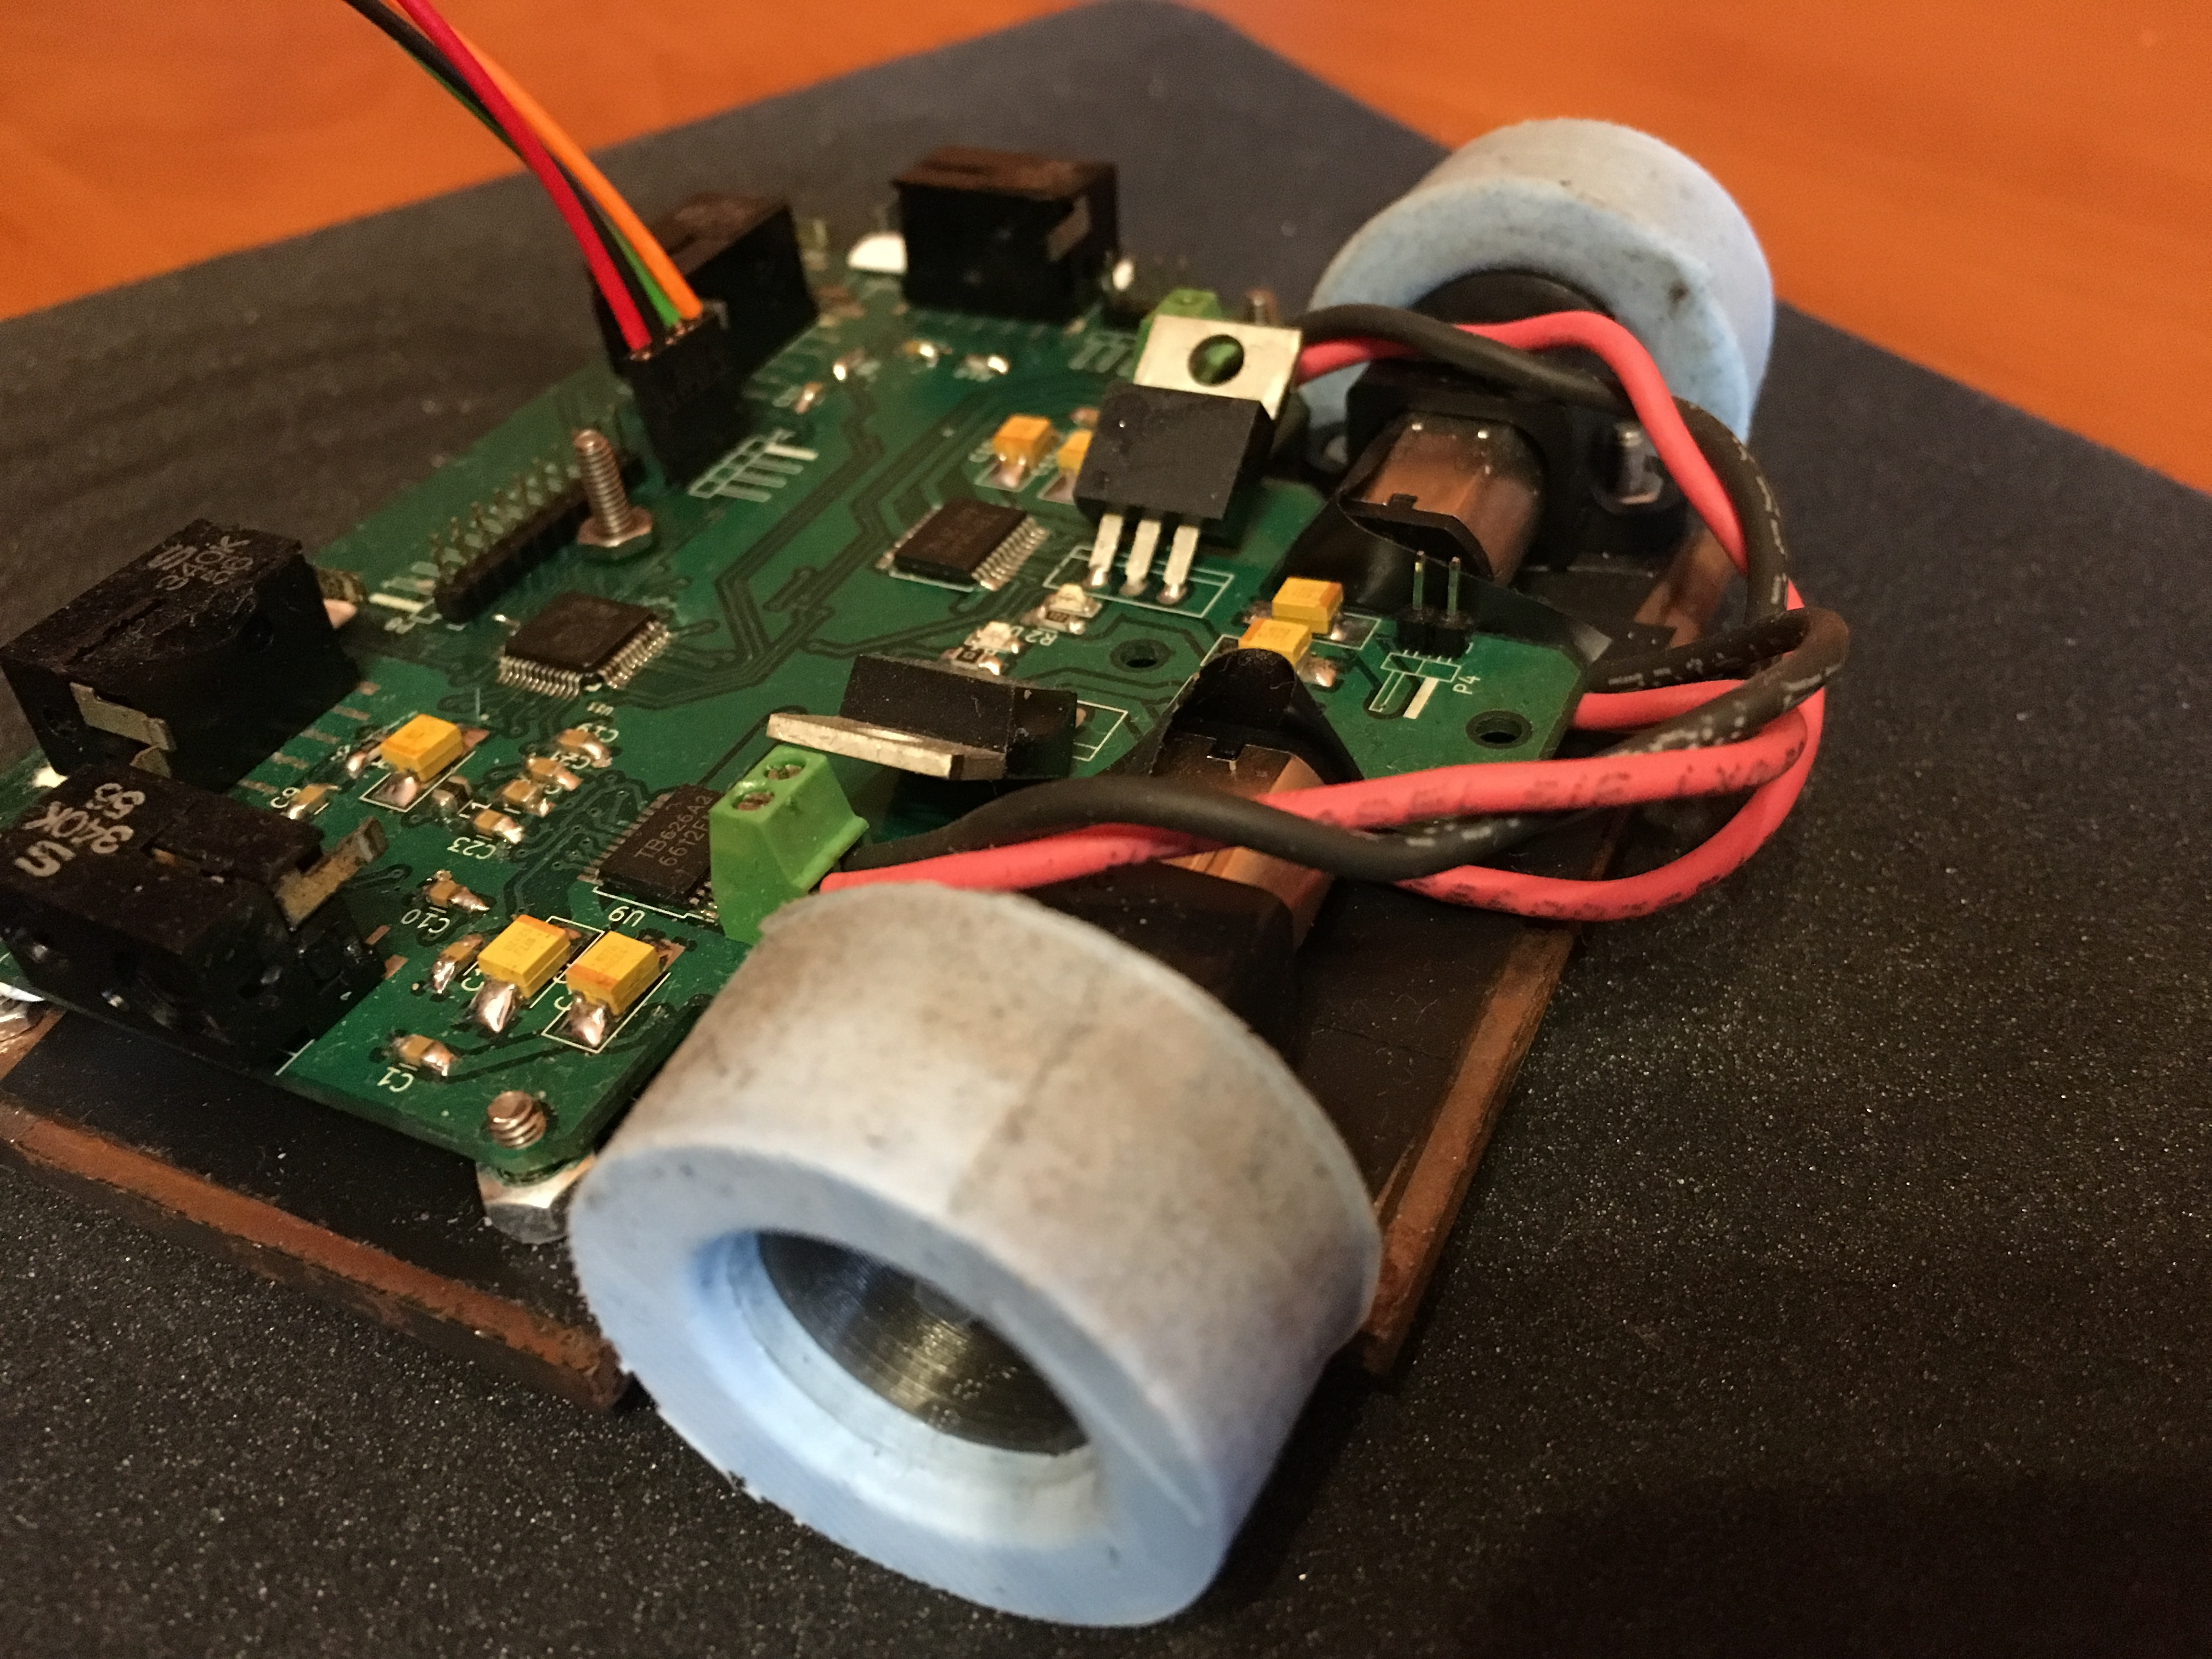
\includegraphics[width=0.75\linewidth]{pic04/drive.JPG}
	\caption{Napęd robota minisumo.}
	\label{fig:drive}	
\end{figure}

Na zdjęciu ~\ref{fig:drive} przedstawiono napęd robota na który składają się dwa silniki oraz dwie felgi z oponami. Jako jednostkę napędową użyto silników \textit{Pololu HPCB} ze względu  na rozmiary, dopuszczalne napięcie zasilania oraz korzystny stosunek ceny do jakości. Felgi zostały wykonane przy pomocy wydruku 3D, a opony były gotowym komponentem wykonanym z poliuretanu.
\section{Elektronika}
Blabla . . .
\subsection{Założenia}
\subsection{Źródło zasilania}
\subsection{Procesor}
\subsection{Sensoryka}
\subsection{Sterownik silników}
\subsection{Schemat płytki z interfejsem}
\subsection{Schemat płytki głównej}

\section{Oprogramowanie}
\subsection{Transmisja danych}
\subsection{Obsługa przychodzących wiadomości}
\subsection{Algorytmy walki}
